%%%%%%%%%%%%%%%%%%%%%%%%%%%%%%%%%%%%%%%%%%
% Engineering problems / LaTeX Template
%		Semester 6
%		Institut d'Optique Graduate School
%%%%%%%%%%%%%%%%%%%%%%%%%%%%%%%%%%%%%%%%%%
%	6N-IntNum-BlocTraitImage	/ Image processing
%%%%%%%%%%%%%%%%%%%%%%%%%%%%%%%%%%%%%%%%%%
%
% Created by:
%	Julien VILLEMEJANE - 16/jul/2024
% Fichier.sty modifié pour changer la police de caractère
%	
%
%%%%%%%%%%%%%%%%%%%%%%%%%%%%%%%%%%%%%%%%%%
% Professional Newsletter Template
% LaTeX Template
% Version 1.0 (09/03/14)
%
% Created by:
% Bob Kerstetter (https://www.tug.org/texshowcase/) and extensively modified by:
% Vel (vel@latextemplates.com)
% 
% This template has been downloaded from:
% http://www.LaTeXTemplates.com
%
% License:
% CC BY-NC-SA 3.0 (http://creativecommons.org/licenses/by-nc-sa/3.0/)
%
%%%%%%%%%%%%%%%%%%%%%%%%%%%%%%%%%%%%%%%%%

\documentclass[a4paper,11pt,titlepage]{article} % The default font size is 10pt; 11pt and 12pt are alternatives

%%%%%%%%%%%%%%%%%%%%%%%%%%%%%%%%%%%%%%%%%%%%%%%%%%%%%%%%%%%%%%%%%%%%%%%%%%%%%%%%%%%%%%%%%%%%%%%%%%%%%%%%%%%%%%%%%%%%%%%%%%%%%%%%%%%%%%%%%%%%%%%%%%%%%%%%%%%%%%%%%%%%%%%%%%%%%%%%%%%%%%%%%%%%%%%%%%%%%%%%%%%%%%%%%%%%%%%%%%%%%%%%%%%%%%%%%%%%%%%%%%%%%%%%%%%%
\usepackage{opto_elec_villemejane}

%%%%%%%%%%%%%%%%%%%%%%%%%%%%%%%%%%%%%%%%%%%%%%%%
%%%%%%%%%%%%%%%%%%%%%%%%%%%%%%%%%%%%%%%%%%%%%%%%
\begin{document}



% Page de garde
\begin{titlepage}

\begin{center}
	\begin{minipage}{2.5cm}
	\begin{center}
		
\includegraphics[width=8cm]{images/Logo-LEnsE.png}
	\end{center}
\end{minipage}\hfill
\begin{minipage}{10cm}
	\begin{center}
	\textbf{Institut d'Optique Graduate School }\\[0.1cm]
    \textbf{Interfaçage Numérique}


	\end{center}
\end{minipage}\hfill


\vspace{4cm}


{\huge \bfseries \textsc{Interfaçage Numérique}} \\[0.5cm]
{\large \bfseries Travaux Pratiques} \\[0.2cm]
Semestre 6

\vspace{2cm}
% Title
\rule{\linewidth}{0.3mm} \\[0.4cm]
{ \huge \bfseries\color{violet_iogs} Développement d'une interface en PyQt6 \\[0.4cm] }
\rule{\linewidth}{0.3mm} \\[1cm]

2 séances

\bigskip

\begin{center}
	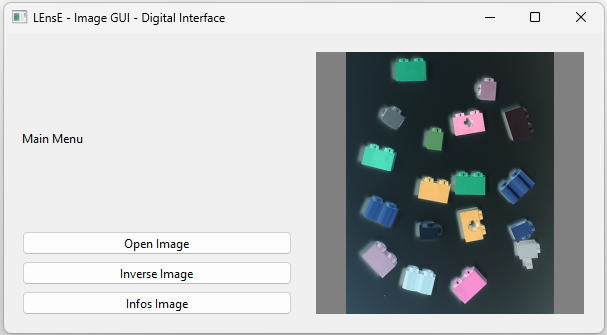
\includegraphics[width=0.5\textwidth]{images/image_gui.png}
\end{center}

\vfill

\textit{Ce sujet est disponible au format électronique sur le site du LEnsE - https://lense.institutoptique.fr/ dans la rubrique Année / Première Année / Interfaçage Numérique S6 / Bloc 2 Caméra, Images et Interfaces / Interface Humain-Machine.}

% Bottom of the page
%{\textbf{\large {Année universitaire} 2024-2025}}

\end{center}
\end{titlepage}

\newpage
\strut % empty page

%%%%%%%%%%%%%%%%%%%%%%%%%%%%%%%%%%%%%%%%%%%%%%%%
%%%%%%%%%%%%%    Intro
\newpage
\pagestyle{empty}

\begin{minipage}[c]{.25\linewidth}
	
\includegraphics[width=5cm]{images/Logo-LEnsE.png}
\end{minipage} \hfill
\begin{minipage}[c]{.4\linewidth}

\begin{center}
\vspace{0.3cm}
{\Large \textsc{Interfaçage Numérique}}

\medskip

6N-047-SCI \qquad \textbf{\Large GUI}

\end{center}
\end{minipage}\hfill

\vspace{0.5cm}

\noindent \rule{\linewidth}{1pt}

{\noindent\Large  \rule[-7pt]{0pt}{30pt} \textbf{Développement d'une Interface en PyQt6}}

\noindent \rule{\linewidth}{1pt}

\bigskip 

%%%%%%%%%%%%%%%%%%%%%%%%%%%%%%%%%%%%%%%%%%%%%%%%
%%%%%%%%%%%%%    A A V

{\large À l'issue des séances de TP concernant le \textbf{bloc de développement d'une interface}, les étudiant$\cdot$es seront capables de \textbf{développer une interface Humain-Machine simple} à partir d'un exemple pour ouvrir une image et afficher le résultat d'un traitement sous forme d'un graphique.}


\noindent \rule{\linewidth}{1pt}

\medskip

Pour cela, ils$\cdot$elles seront capables de~:

\begin{itemize}
	\item \textbf{ajouter des éléments graphiques} à une interface existante ;
	\item \textbf{gérer les événements} liés aux éléments graphiques dynamiques (boutons...) ;
	\item \textbf{afficher un graphique ou une image} dans un conteneur graphique de l'interface.
\end{itemize}


\noindent \rule{\linewidth}{1pt}

\medskip


%%%%%%%%%%%%%%%%%%%%%%%%%%%%%%%%%%%%%%%%%%%%%%%%
%%%%%%%%%%%%%    Objectifs

\section{Objectifs du bloc}

L'objectif principal de ce bloc est de \textbf{réaliser une interface humain-machine permettant d'afficher le résultat d'une simulation simple} ou de données.

Cette interface sera codée à l'aide de la bibliothèque \textbf{PyQt6} et les étudiant$\cdot$es seront amené$\cdot$es à découvrir les éléments de base d'une telle interface.

Cette séquence de TP est basée sur le langage \textbf{Python}. Vous pourrez utiliser l'environnement \textbf{PyCharm} (édition Community 2023 - ou supérieure) et \textbf{Python 3.10} (ou version supérieure - inclus dans la distribution Anaconda 3).

%%%%%%%%%%%%%%%%%%%%%%%%%%%%%%%%%%%%%%%%%%%%%%%%
%%%%%%%%%%%%%    Ressources

\section{Ressources}

Un \textbf{tutoriel sur PyQt6} est disponible à l'adresse suivante :

\href{https://iogs-lense-training.github.io/python-pyqt-gui/}{https://iogs-lense-training.github.io/python-pyqt-gui/}

Des \textbf{codes d'exemple} associés à ce sujet sont disponibles à l'adresse suivante : 

\href{https://lense.institutoptique.fr/ressources/Annee1/InterfacageNumerique/bloc_gui/codes/}{https://lense.institutoptique.fr/ressources/Annee1/InterfacageNumerique/bloc\_gui/codes/}

\medskip

Il existe également une multitude de tutoriaux et d'exemples sur Internet d'application basée sur \textbf{PyQt6}. 

Par exemple :  \href{https://www.pythonguis.com/pyqt6-tutorial/}{https://www.pythonguis.com/pyqt6-tutorial/}.

\medskip

Enfin, n'hésitez pas à vous rendre sur la \textbf{documentation officielle} de Qt pour Python : 

\href{https://doc.qt.io/qtforpython-6/}{https://doc.qt.io/qtforpython-6/}


\newpage
%%%%%%%%%%%%%%%%%%%%%%%%%%%%%%%%%%%%%%%%%%%%%%%%
%%%%%%%%%%%%%    Déroulement
\section{Déroulement du bloc}

Ce bloc se déroule en deux temps :

\begin{itemize}
	\item une première partie où vous serez guidé$\cdot$es pour \textbf{découvrir les éléments de base d'une interface} développée à l'aide de la bibliothèque \textbf{PyQt6}, incluant une gestion des événements ;
	\item une seconde partie où vous serez plus en autonomie pour \textbf{répondre à l'un des sujets proposés} autour de l'\textbf{affichage de données de simulation} ou tout autre traitement de données.
\end{itemize}

\medskip

\subsection{Premiers éléments graphiques et interactions}
	\begin{description}
		\item[Etape 1 - 30 min] Etudier la structure de base d'une application PyQt6 (sans évènement)
		\item[Etape 2 - 30 min] Intégrer de nouveaux éléments graphiques
		\item[Etape 3 - 60 min] Utiliser des signaux pour gérer des évènements
		\item[Etape 4 - 60 min] Ouvrir une image et l'afficher
		\item[Etape 5 - 60 min] Afficher un graphique
	\end{description}
	
	\bigskip
	
\subsection{Affichage de données de simulation ou de traitement}

Le but final est d'afficher des données provenant soit d'un fichier à ouvrir : histogramme d'une image, données dans un fichier CSV... , soit d'une simulation/observation/modélisation : réponse à un échelon, ...

	
\noindent \rule{\linewidth}{1pt}

\newpage
\strut % empty page
%%%%%%%%%%%%%%%%%%%%%%%%%%%%%%%%%%%%%%%%%%%%%%%%
%%%%%%%%%%%%%    Séance 1 détaillée

\begin{minipage}[c]{.25\linewidth}
	
\includegraphics[width=4cm]{images/Logo-LEnsE.png}
\end{minipage} \hfill
\begin{minipage}[c]{.4\linewidth}

\begin{center}
\vspace{0.3cm}
{\Large \textsc{Interfaçage Numérique}}

\medskip

6N-047-SCI \qquad \textbf{\Large Bloc GUI}

\end{center}
\end{minipage}\hfill

\vspace{0.5cm}

\noindent \rule{\linewidth}{1pt}

{\noindent\Large \rule[-7pt]{0pt}{30pt} Premiers éléments graphiques et interactions} 

\noindent \rule{\linewidth}{1pt}


%%%%%%%%%%%%%%%%%%%%%%%%%%%%%%%%%%%%%%%%%%%%%%%%
%%%%%%%%%%%%%    Objectifs
\section{Objectifs de la séance}

Dans cette première partie, vous allez \textbf{étudier des exemples de code} permettant d'afficher certains éléments graphiques dans une IHM \textbf{PyQt6} et de réaliser des actions associées à certains de ces éléments. 

%%%%%%%%%%%%%%%%%%%%%%%%%%%%%%%%%%%%%%%%%%%%%%%%
%%%%%%%%%%%%%    Déroulement détaillé

%%%%%%%%%%%%%    Etape 1
\section{Etudier la structure de base d'une application PyQt6}

\begin{center} \textbf{\textit{Temps conseillé : 30 min}} \end{center}

Dans cette section, vous allez étudier une application simple basée sur PyQt6 afin de \textbf{découvrir les briques élémentaires} à mettre en oeuvre dans ce type d'interface.

\medskip

A partir du fichier \textbf{start\_gui.py} :

\begin{itemize}
	\item Lancer l'application et visualiser le résultat.
	\item Étudier un peu plus en détail la structure du code fourni et notamment les différents types de conteneurs utilisés. Faire un schéma des différents éléments et leurs liens.
\end{itemize}
	

%%%%%%%%%%%%%    Etape 2
\section{Intégrer de nouveaux éléments graphiques}		

\begin{center} \textbf{\textit{Temps conseillé : 30 min}} \end{center}

L'interface précédente n'inclut pas d'objets graphiques interactifs (bouton, zone de sélection...). Nous allons dans cette section \textbf{ajouter quelques boutons}.

A partir du fichier \textbf{start\_gui.py} :

\begin{itemize}
	\item Ajouter un bouton (\textbf{QPushButton}) nommé \textsl{\textbf{first\_button}} au menu principal
	\item Ajouter une action à ce bouton qui appelle la fonction \textsl{\textbf{action\_clicked}} lorsqu'on clique dessus
	\item Ajouter un second bouton nommé \textsl{\textbf{second\_button}} au menu principal, qui appelle la fonction \textsl{\textbf{action\_clicked}} lorsqu'on clique dessus.
	\item Tester votre application.
	
	\medskip	
	
	\item Modifier les actions associées selon le bouton appuyé :
	\begin{itemize}
		\item \textsl{\textbf{first\_button}} : renomme le nom du menu principal ;
		\item \textsl{\textbf{second\_button}} : renomme le nom de la fenêtre principale.
	\end{itemize}
\end{itemize}

\newpage
%%%%%%%%%%%%%    Etape 3
\section{Utiliser des signaux pour gérer des évènements}

\begin{center} \textbf{\textit{Temps conseillé : 60 min}} \end{center}

Avec la structure précédente, il est nécessaire que les éléments graphiques contenus dans un \textbf{QWidget}, par exemple, connaissent l'élément graphique dit parent afin de pouvoir interagir avec celui-ci.

Une autre méthode consiste à utiliser des signaux (objet de la classe \textbf{pyQtSignal}) pour transmettre des informations d'un objet à un autre. L'exemple suivant propose d'étudier cette méthode.

A partir du fichier \textbf{signal\_gui.py}

\begin{itemize}
	\item Lancer l'application et visualiser le résultat.
	\item Étudier la nouvelle structure et trouver les points communs et les différences avec la précédente structure de code.
	
	\medskip
	
	\item Ajouter une fonction \textsl{\textbf{set\_title}} à la classe \textbf{MainWidget} pour modifier le titre de la section principale
	\item Modifier l'application pour obtenir les mêmes interactions que précédemment avec les deux boutons, mais sans modifier la fonction \textsl{\textbf{action\_clicked}} de la classe \textbf{MainMenuWidget}
\end{itemize}


%%%%%%%%%%%%%    Etape 4
\section{Ouvrir une image et l'afficher}

\begin{center} \textbf{\textit{Temps conseillé : 30 min}} \end{center}

Il est parfois utile que l'utilisateur$cdot$trice puisse ouvrir un fichier. Nous allons ici nous intéresser à l'ouverture et l'affichage d'un fichier contenant une image (type \textit{jpg}).

A partir du fichier \textbf{image\_gui.py}

\begin{itemize}
	\item Lancer l'application et visualiser le résultat.
	\item Ouvrir une image à l'aide de l'interface.
	\item Étudier la structure de l'application proposée, notamment les liens entre les différentes classes.

	\medskip	
	
	\item Ajouter un bouton dans le menu principal permettant d'inverser l'affichage des couleurs de l'image et modifier le code pour que l'affichage soit mis à jour.
	\item Ajouter un bouton dans le menu principal permettant d'afficher dans la console la taille de l'image et la moyenne de l'ensemble de ses pixels.
	\item Modifier le code de l'application pour que les boutons d'inversion et d'affichage des informations de l'image soit par défaut non utilisable et qu'ils le deviennent uniquement lorsqu'une image est chargée.
	\item BONUS : Modifier le comportement du bouton d'affichage des informations pour qu'il affiche en plus l'histogramme (pour les 3 couleurs de l'image) dans une fenêtre Matplotlib classique (hors interface pyQt6).
\end{itemize}

\newpage
%%%%%%%%%%%%%    Etape 5
\section{Afficher un graphique}

\begin{center} \textbf{\textit{Temps conseillé : 60 min}} \end{center}

Dans cette section, nous allons nous intéresser à l'affichage et la mise à jour d'un graphique à l'intérieur d'un conteneur graphique.

\begin{center}
	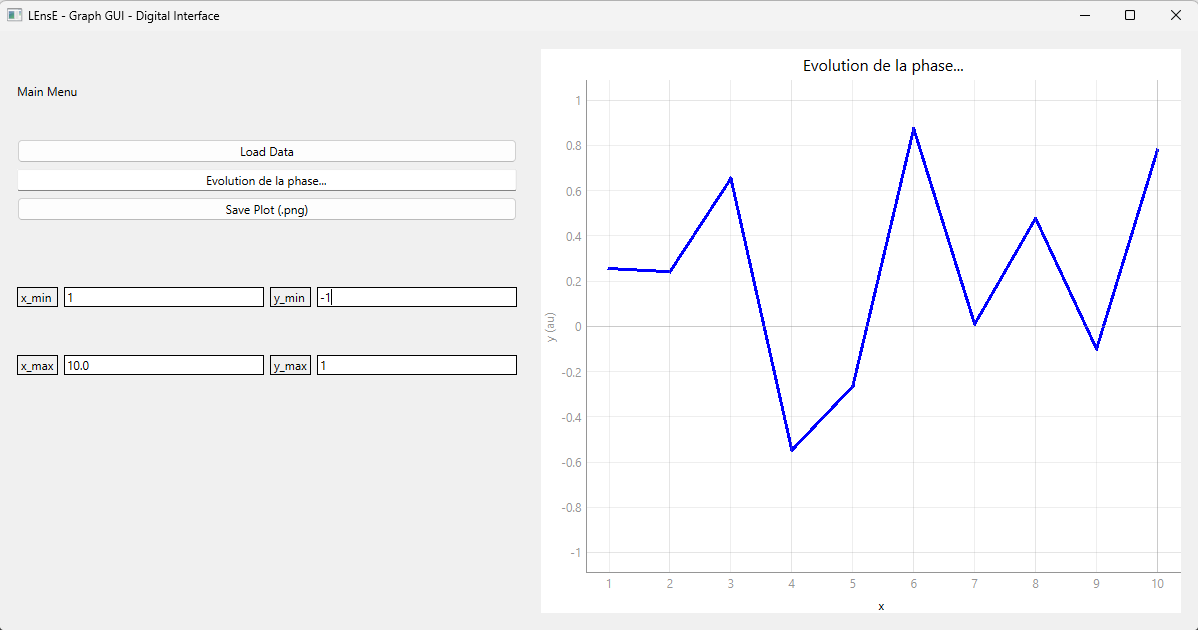
\includegraphics[width=0.6\textwidth]{images/graph_gui.png}
\end{center}


A partir du fichier \textbf{graph\_gui.py}

\begin{itemize}
	\item Lancer l'application et visualiser le résultat en chargeant les données du fichier \textbf{data.csv} fourni
	\item Modifier la couleur du fond du graphique ainsi que l'épaisseur et la couleur d'affichage de la courbe.
	\item Désactiver l'utilisation du bouton \textit{Save Plot (.png)} par défaut et autoriser la sauvegarde lorsque des données sont présentes.
\end{itemize}

\medskip

On se propose maintenant de pouvoir \textbf{interagir avec le graphique} en permettant d'en changer certains paramètres (limites d'affichage en X et en Y).

Une classe \textbf{RangeWidget}, qu'il faudra compléter, a été conçue à cet effet. Des zones de texte ont été prévues pour saisir les limites d'affichage en X et en Y du graphique. Ces zones ne sont pas éditables tant que des données n'ont pas été chargées.

\begin{itemize}
	\item Ajouter un objet de type \textbf{RangeWidget} dans le menu principal.
	\item Modifier le code pour activer les zones de texte ($x\_min$, $x\max$...) lors du chargement des données.
	\item Ajouter une méthode \textsl{\textbf{set\_lim}} à la classe \textbf{RangeWidget} permettant de mettre à jour les limites des axes du graphique. \textit{Les zones de texte fournissent des chaines de caractères et non des nombres...}
	
	\medskip
	
	\item Modifier le code pour que la fonction \textsl{\textbf{set\_lim}} soit appelée à chaque fois que les zones de texte sont modifiées par l'utilisateur$cdot$trice. \textit{Indice : utilisation de la méthode \textsl{\textbf{setRange}} de \textbf{pyQtGraph} et du signal \textsl{\textbf{textChanged}} de \textbf{QLineEdit}.}
	
	\item Ajouter une zone de texte (\textbf{QLineEdit}) dans le menu principal permettant de modifier le titre du graphique.
	\item Modifier le code pour que la sauvegarde du graphique sous forme d'une image PNG soit faite dans un fichier qui porte le titre du graphique.
	
\end{itemize}


\newpage
\strut % empty page
%%%%%%%%%%%%%%%%%%%%%%%%%%%%%%%%%%%%%%%%%%%%%%%%
%%%%%%%%%%%%%    Séance 2 détaillée

\begin{minipage}[c]{.25\linewidth}
	
\includegraphics[width=4cm]{images/Logo-LEnsE.png}
\end{minipage} \hfill
\begin{minipage}[c]{.4\linewidth}

\begin{center}
\vspace{0.3cm}
{\Large \textsc{Interfaçage Numérique}}

\medskip

6N-047-SCI \qquad \textbf{\Large Bloc GUI}

\end{center}
\end{minipage}\hfill

\vspace{0.5cm}

\noindent \rule{\linewidth}{1pt}

{\noindent\Large \rule[-7pt]{0pt}{30pt} Affichage de données de simulation} 

\noindent \rule{\linewidth}{1pt}

%%%%%%%%%%%%%%%%%%%%%%%%%%%%%%%%%%%%%%%%%%%%%%%%
%%%%%%%%%%%%%    Sujets et objectifs

Vous devrez traiter l'un des sujets suivants, \textbf{au choix}.


\section{Sujet A : Filtrage par TF}

A partir du fichier \textbf{image\_filter\_gui.py}, on souhaite pouvoir :

\begin{itemize}
	\item ouvrir une image,
	\item calculer la TF de cette image (FFT2D),
	\item créer un masque sur la TF (circulaire par exemple ou rectangulaire),
	\item générer l'image résultante (par TF inverse) et l'afficher.
\end{itemize}

\textit{Ce sujet peut-être mis en lien avec le TP de filtrage en Optique S6.}


\section{Sujet B : Masque sur une image}

A partir du fichier \textbf{draw\_mask\_gui.py}, on souhaite pouvoir :
\begin{itemize}
	\item créer un masque rectangulaire à partir de deux points sélectionnés à la souris,
	\item stocker le masque dans une matrice de la même taille que l'image,
	\item afficher l'image avec le masque dans une nouvelle fenêtre,
	\item calculer l'histogramme des deux images et les afficher (pour les comparer).
\end{itemize}

\medskip

Il est possible d'accélérer le traitement des calculs par l'utilisation d'une matrice \textit{Numpy} qui ne prend pas en compte les valeurs qui ne sont pas incluses dans le masque : 

\begin{lstlisting}
new_image = np.ma.masked_where(np.logical_not(mask), image)
\end{lstlisting}

L'objet \textsl{mask} doit contenir des données de type booléen.



\section{Sujet C : Coupe dans une image}

A partir du fichier \textbf{image\_slicer\_gui.py}, on souhaite pouvoir :

\begin{itemize}
	\item ouvrir une image,
	\item spécifier une ligne (ou une colonne particulière) selon laquelle on souhaite avoir une coupe de l'image,
	\item afficher la coupe de l'image selon la ligne (ou colonne) sélectionnée.
\end{itemize}

\textit{Cette méthode est utilisée pour analyser des images ayant un profil particulier : faisceau laser (projet en ONIP-1), tâche de diffraction (TP d'Optique S6 - comparaison avec une fonction de Bessel)...}

	
%%%%%%%%%%%%%%%%%%%%%%%%%%%%%%%%%%%%%%%%%%%%%%%%
%%% RESSOURCES COMPLEMENTAIRES	
%
%\newpage
%% Ressources
%\begin{center}
%	\begin{minipage}{2.5cm}
%	\begin{center}
%		
\includegraphics[width=5cm]{images/Logo-LEnsE.png}
%	\end{center}
%\end{minipage}\hfill
%\begin{minipage}{10cm}
%	\begin{center}
%	\textbf{Institut d'Optique Graduate School }\\[0.1cm]
%    \textbf{Interfaçage Numérique}
%
%
%	\end{center}
%\end{minipage}\hfill
%
%
%\vspace{2cm}
%
%
%{\Large \bfseries \textsc{Interfaçage Numérique}} \\[0.5cm]
%{\large \bfseries Travaux Pratiques} \\[0.2cm]
%Semestre 6
%
%\vspace{1cm}
%
%% Title
%\rule{\linewidth}{0.4mm} \\[0.4cm]
%{ \Large \bfseries\color{violet_iogs} Ressources \\[0.4cm] }
%\rule{\linewidth}{0.4mm} \\[1cm]
%{\large Bloc Trait. Image}
%
%\end{center}
%
%\vspace{3cm}
%
%\textbf{\large Liste des ressources}
%\begin{itemize}
%	\item ?
%\end{itemize}
%
%\vfill
%
%\newpage
%\strut % empty page
%
%
%%\includepdf[pages=2, pagecommand={\section{\texorpdfstring{\hspace{-1em}}{Doc Led Rouge}}}\label{doc:ledRouge}]{ressources/kingbright_LED_Rouge.pdf}
%%\includepdf[pages=3]{ressources/kingbright_LED_Rouge.pdf}

\end{document}


